\section{Riemann Integration} 

  We have done integration over closed intervals $[a, b]$. The natural extension is to define integration over \textit{boxes} $B = \prod_i [a_i, b_i]$. Essentially the construction is exactly the same. 

  \begin{definition}[Partition/Mesh]
    Let $B = \prod_i [a_i, b_i] \subset \mathbb{R}^n$ be a \textit{box}. Then, a \textbf{partition}---or \textbf{mesh}---of $B$ is a finite set of points $P = \{x_{ij}\}_{1 \leq i \leq n, 0 \leq j \leq m_i}$\footnote{Therefore, for each dimension $i$, we want to take the interval $[a_i, b_i]$ and subdivide it into $m_i+1$ subintervals.} s.t. 
    \begin{equation}
      a_i = x_{i, 0} \leq x_{i, 1} \leq x_{i, 2} \leq \ldots \leq x_{i, m_i-1} \leq x_{i, m_i} = b \quad \forall i = 1, \ldots, n
    \end{equation}
    We denote each \textbf{box} within the partition as 
    \begin{equation}
      \Delta_j = \Delta_{j_1, j_2, \ldots, j_n} = \prod_{i} [x_{i, j_k-1}, x_{i, j_k}] \quad \forall j_i = 1, \ldots, m_i
    \end{equation}
    of volume $|\Delta_j| \coloneqq \prod_{i} (x_{i, j_k} - x_{i, j_{k-1}})$. 
  \end{definition}

  This nearly\footnote{since boundaries overlap} partitions $B$ into a grid of $\prod_i m_i$ smaller boxes, and can be seen as a discretization of the integral which we will construcct. 

  \begin{definition}[Darboux Sums with Respect to Partition]
		Let $f: E \subset \mathbb{R}^n \to \mathbb{R}$ be a bounded function, let $B \subset E$ be a box, and $P$ be a partition of $B$. Then, the \textbf{upper and lower Darboux integrals} of $f$ with respect to $P$ are defined 
    \begin{equation}
      U(P, f) \coloneqq \sum_{J} \sup_{x \in \Delta_J} f(x) |\Delta_J|, \qquad L(P, f) \coloneqq \sum_{J} \inf_{x \in \Delta_J} f(x) |\Delta_J|
    \end{equation}

    \begin{figure}[H]
      \centering
      \begin{subfigure}[b]{0.48\textwidth}
        \centering
        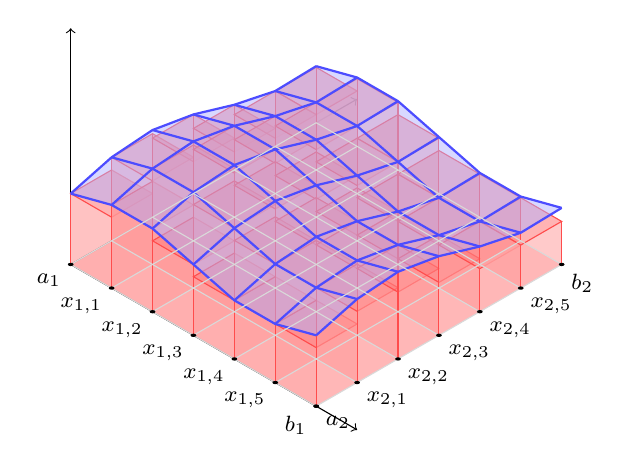
\begin{tikzpicture}[scale=0.6,
          x={(0.866cm,-0.5cm)}, y={(0.866cm,0.5cm)}, z={(0cm,1cm)}]
          
          % Draw axes (without labels)
          \draw[->] (0,0,0) -- (7,0,0);
          \draw[->] (0,0,0) -- (0,7,0);
          \draw[->] (0,0,0) -- (0,0,5);
          
          % Draw rectangular prisms (lower Riemann sum)
          % Using minimum z-value in each cell for lower sum
          \foreach \x in {0,1,2,3,4,5} {
            \foreach \y in {0,1,2,3,4,5} {
              % Calculate heights at four corners of the cell
              \pgfmathsetmacro{\zaa}{1.5 + 0.3*sin(\x*60) + 0.35*sin(\y*50)}
              \pgfmathsetmacro{\zba}{1.5 + 0.3*sin((\x+1)*60) + 0.35*sin(\y*50)}
              \pgfmathsetmacro{\zbb}{1.5 + 0.3*sin((\x+1)*60) + 0.35*sin((\y+1)*50)}
              \pgfmathsetmacro{\zab}{1.5 + 0.3*sin(\x*60) + 0.35*sin((\y+1)*50)}
              
              % Find minimum height (lower Riemann sum)
              \pgfmathsetmacro{\zmin}{min(\zaa,min(\zba,min(\zbb,\zab)))}
              
              % Bottom face (on xy-plane)
              \fill[red!30, opacity=0.6] (\x,\y,0) -- (\x+1,\y,0) -- (\x+1,\y+1,0) -- (\x,\y+1,0) -- cycle;
              
              % Front face
              \fill[red!40, opacity=0.6] (\x,\y,0) -- (\x+1,\y,0) -- (\x+1,\y,\zmin) -- (\x,\y,\zmin) -- cycle;
              
              % Right face
              \fill[red!35, opacity=0.6] (\x+1,\y,0) -- (\x+1,\y+1,0) -- (\x+1,\y+1,\zmin) -- (\x+1,\y,\zmin) -- cycle;
              
              % Top face
              \fill[red!50, opacity=0.6] (\x,\y,\zmin) -- (\x+1,\y,\zmin) -- (\x+1,\y+1,\zmin) -- (\x,\y+1,\zmin) -- cycle;
              
              % Draw edges
              \draw[red!70] (\x,\y,0) -- (\x,\y,\zmin);
              \draw[red!70] (\x+1,\y,0) -- (\x+1,\y,\zmin);
              \draw[red!70] (\x+1,\y+1,0) -- (\x+1,\y+1,\zmin);
              \draw[red!70] (\x,\y+1,0) -- (\x,\y+1,\zmin);
              \draw[red!70] (\x,\y,\zmin) -- (\x+1,\y,\zmin) -- (\x+1,\y+1,\zmin) -- (\x,\y+1,\zmin) -- cycle;
            }
          }
          
          % Draw surface patches first (back to front for proper layering)
          \foreach \ystart/\yend in {0/1, 1/2, 2/3, 3/4, 4/5, 5/6} {
            \foreach \xstart/\xend in {0/1, 1/2, 2/3, 3/4, 4/5, 5/6} {
              \pgfmathsetmacro{\zaa}{1.5 + 0.3*sin(\xstart*60) + 0.35*sin(\ystart*50)}
              \pgfmathsetmacro{\zba}{1.5 + 0.3*sin(\xend*60) + 0.35*sin(\ystart*50)}
              \pgfmathsetmacro{\zbb}{1.5 + 0.3*sin(\xend*60) + 0.35*sin(\yend*50)}
              \pgfmathsetmacro{\zab}{1.5 + 0.3*sin(\xstart*60) + 0.35*sin(\yend*50)}
              
              \fill[blue!30, opacity=0.5] 
                (\xstart,\ystart,\zaa) --
                (\xend,\ystart,\zba) --
                (\xend,\yend,\zbb) --
                (\xstart,\yend,\zab) -- cycle;
            }
          }
          
          % Draw grid lines on surface
          % Lines parallel to x-axis
          \foreach \y in {0,1,2,3,4,5,6} {
            \draw[blue!70, thick] 
              (0,\y,{1.5 + 0.35*sin(\y*50)}) 
              \foreach \x in {1,2,3,4,5,6} {
                -- (\x,\y,{1.5 + 0.3*sin(\x*60) + 0.35*sin(\y*50)})
              };
          }
          
          % Lines parallel to y-axis
          \foreach \x in {0,1,2,3,4,5,6} {
            \draw[blue!70, thick] 
              (\x,0,{1.5 + 0.3*sin(\x*60)}) 
              \foreach \y in {1,2,3,4,5,6} {
                -- (\x,\y,{1.5 + 0.3*sin(\x*60) + 0.35*sin(\y*50)})
              };
          }
          
          % Base grid
          \foreach \x in {0,1,2,3,4,5,6} {
            \draw[gray!30, thin] (\x,0,0) -- (\x,6,0);
            \draw[gray!30, thin] (0,\x,0) -- (6,\x,0);
          }
          
          % X-axis tick labels (back axis)
          \foreach \x/\label in {0/a_1, 1/x_{1,1}, 2/x_{1,2}, 3/x_{1,3}, 4/x_{1,4}, 5/x_{1,5}, 6/b_1} {
            \fill (\x,0,0) circle (0.05);
            \node[below left, font=\footnotesize] at (\x,0,0) {$\label$};
          }
          
          % Y-axis tick labels (front axis at x=6)
          \foreach \y/\label in {0/a_2, 1/x_{2,1}, 2/x_{2,2}, 3/x_{2,3}, 4/x_{2,4}, 5/x_{2,5}, 6/b_2} {
            \fill (6,\y,0) circle (0.05);
            \node[below right, font=\footnotesize] at (6,\y,0) {$\label$};
          }
        \end{tikzpicture}
        \caption{Lower Riemann sum.}
        \label{fig:lower_riemann_sum}
      \end{subfigure}
      \hfill 
      \begin{subfigure}[b]{0.48\textwidth}
        \centering
        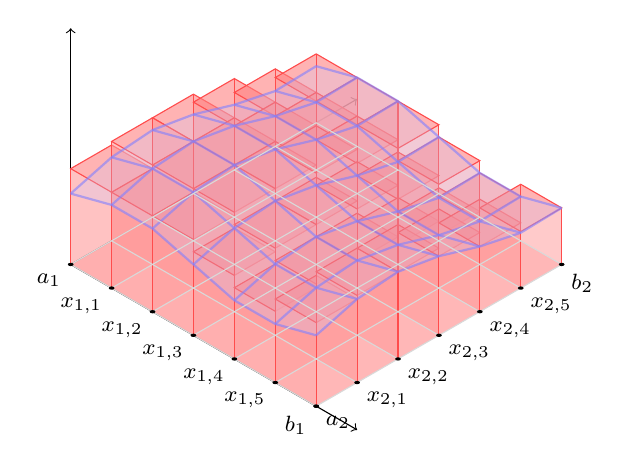
\begin{tikzpicture}[scale=0.6,
          x={(0.866cm,-0.5cm)}, y={(0.866cm,0.5cm)}, z={(0cm,1cm)}]
          
          % Draw axes (without labels)
          \draw[->] (0,0,0) -- (7,0,0);
          \draw[->] (0,0,0) -- (0,7,0);
          \draw[->] (0,0,0) -- (0,0,5);
          
          % Draw rectangular prisms (upper Riemann sum)
          % Using maximum z-value in each cell for upper sum
          \foreach \x in {0,1,2,3,4,5} {
            \foreach \y in {0,1,2,3,4,5} {
              % Calculate heights at four corners of the cell
              \pgfmathsetmacro{\zaa}{1.5 + 0.3*sin(\x*60) + 0.35*sin(\y*50)}
              \pgfmathsetmacro{\zba}{1.5 + 0.3*sin((\x+1)*60) + 0.35*sin(\y*50)}
              \pgfmathsetmacro{\zbb}{1.5 + 0.3*sin((\x+1)*60) + 0.35*sin((\y+1)*50)}
              \pgfmathsetmacro{\zab}{1.5 + 0.3*sin(\x*60) + 0.35*sin((\y+1)*50)}
              
              % Find maximum height (upper Riemann sum)
              \pgfmathsetmacro{\zmax}{max(\zaa,max(\zba,max(\zbb,\zab)))}
              
              % Bottom face (on xy-plane)
              \fill[red!30, opacity=0.6] (\x,\y,0) -- (\x+1,\y,0) -- (\x+1,\y+1,0) -- (\x,\y+1,0) -- cycle;
              
              % Front face
              \fill[red!40, opacity=0.6] (\x,\y,0) -- (\x+1,\y,0) -- (\x+1,\y,\zmax) -- (\x,\y,\zmax) -- cycle;
              
              % Right face
              \fill[red!35, opacity=0.6] (\x+1,\y,0) -- (\x+1,\y+1,0) -- (\x+1,\y+1,\zmax) -- (\x+1,\y,\zmax) -- cycle;
              
              % Top face
              \fill[red!50, opacity=0.6] (\x,\y,\zmax) -- (\x+1,\y,\zmax) -- (\x+1,\y+1,\zmax) -- (\x,\y+1,\zmax) -- cycle;
              
              % Draw edges
              \draw[red!70] (\x,\y,0) -- (\x,\y,\zmax);
              \draw[red!70] (\x+1,\y,0) -- (\x+1,\y,\zmax);
              \draw[red!70] (\x+1,\y+1,0) -- (\x+1,\y+1,\zmax);
              \draw[red!70] (\x,\y+1,0) -- (\x,\y+1,\zmax);
              \draw[red!70] (\x,\y,\zmax) -- (\x+1,\y,\zmax) -- (\x+1,\y+1,\zmax) -- (\x,\y+1,\zmax) -- cycle;
            }
          }
          
          % Draw surface patches with lighter opacity
          \foreach \ystart/\yend in {0/1, 1/2, 2/3, 3/4, 4/5, 5/6} {
            \foreach \xstart/\xend in {0/1, 1/2, 2/3, 3/4, 4/5, 5/6} {
              \pgfmathsetmacro{\zaa}{1.5 + 0.3*sin(\xstart*60) + 0.35*sin(\ystart*50)}
              \pgfmathsetmacro{\zba}{1.5 + 0.3*sin(\xend*60) + 0.35*sin(\ystart*50)}
              \pgfmathsetmacro{\zbb}{1.5 + 0.3*sin(\xend*60) + 0.35*sin(\yend*50)}
              \pgfmathsetmacro{\zab}{1.5 + 0.3*sin(\xstart*60) + 0.35*sin(\yend*50)}
              
              \fill[blue!20, opacity=0.25] 
                (\xstart,\ystart,\zaa) --
                (\xend,\ystart,\zba) --
                (\xend,\yend,\zbb) --
                (\xstart,\yend,\zab) -- cycle;
            }
          }
          
          % Draw grid lines on surface (lighter)
          % Lines parallel to x-axis
          \foreach \y in {0,1,2,3,4,5,6} {
            \draw[blue!50, thick, opacity=0.6] 
              (0,\y,{1.5 + 0.35*sin(\y*50)}) 
              \foreach \x in {1,2,3,4,5,6} {
                -- (\x,\y,{1.5 + 0.3*sin(\x*60) + 0.35*sin(\y*50)})
              };
          }
          
          % Lines parallel to y-axis
          \foreach \x in {0,1,2,3,4,5,6} {
            \draw[blue!50, thick, opacity=0.6] 
              (\x,0,{1.5 + 0.3*sin(\x*60)}) 
              \foreach \y in {1,2,3,4,5,6} {
                -- (\x,\y,{1.5 + 0.3*sin(\x*60) + 0.35*sin(\y*50)})
              };
          }
          
          % Base grid
          \foreach \x in {0,1,2,3,4,5,6} {
            \draw[gray!30, thin] (\x,0,0) -- (\x,6,0);
            \draw[gray!30, thin] (0,\x,0) -- (6,\x,0);
          }
          
          % X-axis tick labels (back axis)
          \foreach \x/\label in {0/a_1, 1/x_{1,1}, 2/x_{1,2}, 3/x_{1,3}, 4/x_{1,4}, 5/x_{1,5}, 6/b_1} {
            \fill (\x,0,0) circle (0.05);
            \node[below left, font=\footnotesize] at (\x,0,0) {$\label$};
          }
          
          % Y-axis tick labels (front axis at x=6)
          \foreach \y/\label in {0/a_2, 1/x_{2,1}, 2/x_{2,2}, 3/x_{2,3}, 4/x_{2,4}, 5/x_{2,5}, 6/b_2} {
            \fill (6,\y,0) circle (0.05);
            \node[below right, font=\footnotesize] at (6,\y,0) {$\label$};
          }
        \end{tikzpicture}
        \caption{Upper Riemann sum.}
        \label{fig:upper_riemann_rum}
      \end{subfigure}
      \caption{}
    \end{figure}
  \end{definition}

  \begin{definition}[Darboux Integral]
		Let $f: E \subset \mathbb{R}^n \to \mathbb{R}$ be a bounded function, and let $B \subset E$ be a box. Then, the \textbf{upper and lower Darboux integrals} of $f$ are defined 
    \begin{equation}
      \overline{\int_B} f(x) \,dx \coloneqq \inf_P U(P, f), \qquad \underline{\int_B} f(x) \,dx \coloneqq \sup_P L(P, f) 
    \end{equation}
    If the upper and lower Riemann integrals are equal then $f$ is said to be \textbf{Darboux integrable} over $B$ and the \textbf{Darboux integral} of $f$ is 
    \begin{equation}
      \int_B f(x) \,dx 
    \end{equation}
  \end{definition} 

	\begin{figure}[H]
		\centering
		\begin{subfigure}[b]{0.48\textwidth}
			\centering
			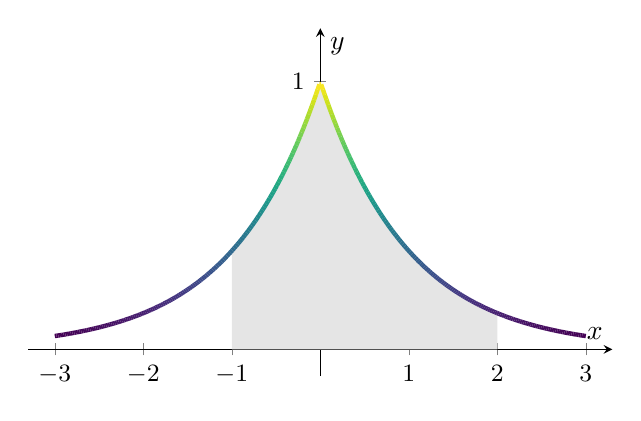
\begin{tikzpicture}
				\begin{axis}[
					axis lines=middle,
					xlabel={$x$},
					ylabel={$y$},
					xmin=-3.3, xmax=3.3,
					ymin=-0.1, ymax=1.2,
					xtick={-3, -2, -1, 0, 1, 2, 3},
					ytick={0.5, 1.0},
					tick label style={font=\small},
					width=9cm,
					height=6cm,
					colormap/viridis, % Sets the color palette gradient
					enlargelimits=false
				]
					% 1. Shaded region under the curve from x = -1 to x = 2
					\addplot[
						fill=gray!20,
						draw=none,
						domain=-1:2,
						samples=100
					] {exp(-abs(x))} \closedcycle;

					% 2. The main curve colored dynamically by height (y-value)
					\addplot[
						mesh,            % Tells pgfplots to color line segments individually
						point meta=y,    % Uses the y-value (height) to determine the color
						ultra thick,     % Thickened slightly so the color changes are easy to see
						domain=-3:3,
						samples=300       % High sampling ensures a smooth color transition
					] {exp(-abs(x))};
				\end{axis}
			\end{tikzpicture}
			\caption{}
		\end{subfigure}
		\hfill 
		\begin{subfigure}[b]{0.48\textwidth}
			\centering
			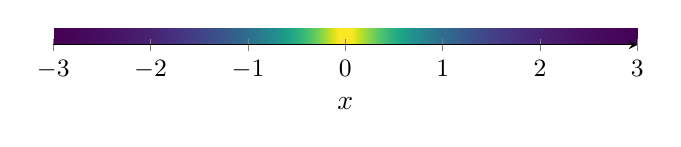
\begin{tikzpicture}
				\begin{axis}[
					view={0}{90}, % Top-down 2D view to flatten the mesh into a strip
					colormap/viridis,
					xlabel={$x$},
					xmin=-3, xmax=3,
					% Tighter y boundaries to make the color strip thin and compact
					ymin=-0.05, ymax=0.05,
					hide y axis,
					axis x line=bottom,
					xtick={-3, -2, -1, 0, 1, 2, 3},
					xticklabel style={font=\small},
					width=9cm,
					height=1.8cm, % Compressed height to look like a thick line
				]
					% Evaluates f(x) = exp(-x) across the horizontal line strip
					\addplot3[
						surf,
						shader=interp,
						domain=-3:3,
						domain y=-0.05:0.05,
						samples=50,
						samples y=2
					] {exp(-abs(x))};
				\end{axis}
			\end{tikzpicture}
			\caption{}
		\end{subfigure}
		\caption{Two interpretations of the integral $\int_{-1}^2 e^{-|x|}\,dx$. On the left, we view it as the area under a curve. On the right, we view it as the mass of a 1-dimensinoal rod lying on $[-1, 2]$ of varying density defined by function $f(x)$.}
		\label{fig:interpretations_of_single_integral}
	\end{figure}

	\begin{figure}[H]
	  \centering
	  \begin{subfigure}[b]{0.48\textwidth}
	    \centering
			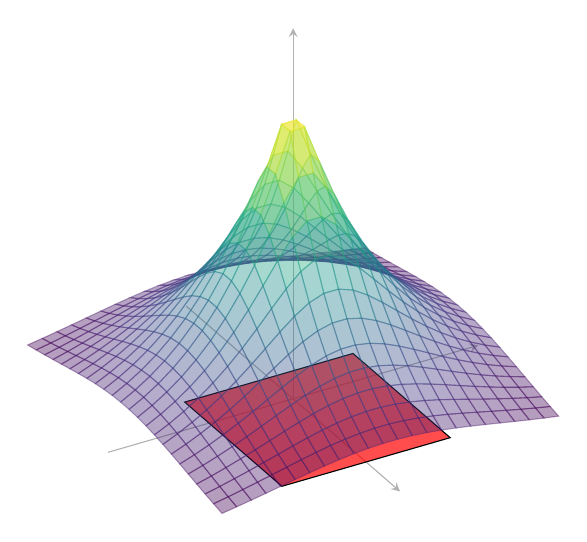
\begin{tikzpicture}
				\begin{axis}[
					view={60}{30}, % 3D projection view angle
					axis lines=center,
					xtick=\empty,
					ytick=\empty,
					ztick=\empty,
					xmin=-2.2, xmax=2.2,
					ymin=-2.2, ymax=2.2,
					zmin=0, zmax=1.2,
					domain=-2:2,
					y domain=-2:2,
					samples=24,
					samples y=24,
					width=9cm,
					height=10.0cm,
					colormap/viridis, % Applied viridis colormap
					shader=flat,
					draw=black!30,
				]
					\draw[
						draw=black,
						solid,
						thin,
						fill=red,
						fill opacity=0.7,
					] (axis cs:-0.5, -1.0, 0) -- (axis cs:1.5, -1.0, 0) 
						 -- (axis cs:1.5, 1.0, 0) -- (axis cs:-0.5, 1.0, 0) -- cycle;

					% 1. The 3D Gaussian Surface (Slightly opaque)
					\addplot3[
						surf,
						opacity=0.4,
					] {exp(-sqrt(x^2 + y^2))};
				\end{axis}
			\end{tikzpicture}
	    \caption{}
	  \end{subfigure}
	  \hfill 
	  \begin{subfigure}[b]{0.48\textwidth}
	    \centering
			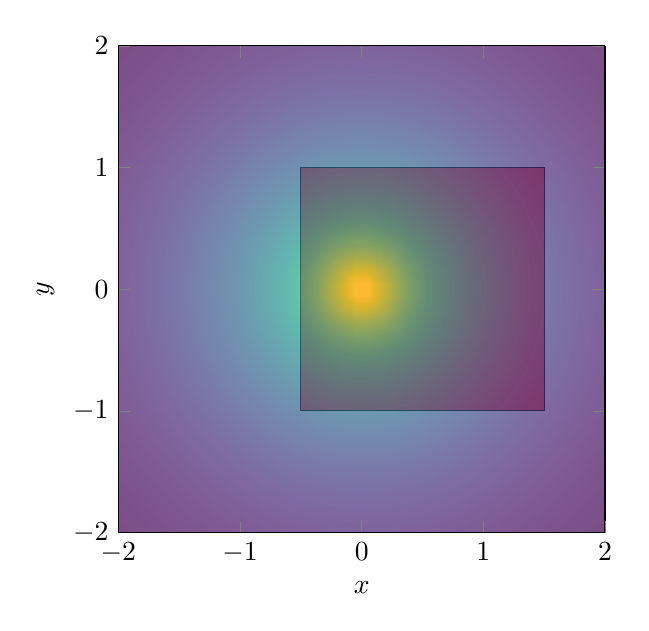
\begin{tikzpicture}
				\begin{axis}[
					view={0}{90},
					colormap/viridis, 
					xlabel={$x$},
					ylabel={$y$},
					xmin=-2, xmax=2,
					ymin=-2, ymax=2,
					zmin=0, zmax=1,
					axis equal image,
					width=9cm,
				]
					\draw[
						draw=black,
						solid,
						thin,
						fill=red,
						fill opacity=0.7,
					] (axis cs:-0.5, -1.0, 1.0) rectangle (axis cs:1.5, 1.0, 1.0);

					\addplot3[
						surf,
						shader=interp,
						domain=-2:2,
						domain y=-2:2,
						samples=40,
						fill opacity=0.7,
					] {exp(-(sqrt(x^2 + y^2)))};

				\end{axis}
			\end{tikzpicture}
	  \end{subfigure}
		\caption{Two interpretations of double integral $\iint_B e^{-\sqrt{x^2 + y^2}} \,dx$. On the left, we can view it as the area under a surface. On the right, we view it as the mass of a 2-dimensional sheet lying on $[-0.5, 1.5] \times [-1, 1]$ of varying density defined by function $f(x, y)$.}
	  \label{fig:interpretations_of_double_integral}
	\end{figure}

\subsection{Conditions for Integrability} 

  \begin{theorem}[Continuous Implies Integrable]
    $f: E \subset \mathbb{R}^n \to \mathbb{R}$ continuous means $f$ is integrable over $B$. 
  \end{theorem}
	\begin{proof}
	  
	\end{proof}

  However, there are some functions with discontinuities that are in fact integrable. 

  \begin{figure}[H]
    \centering
    \begin{subfigure}[b]{0.48\textwidth}
      \centering
      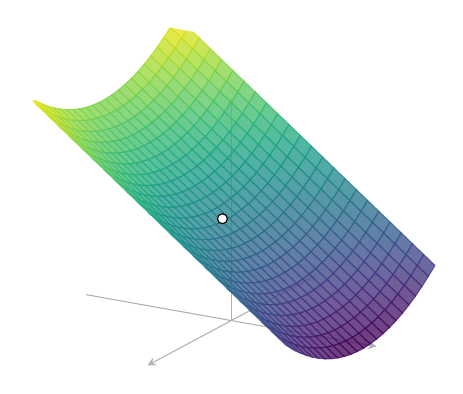
\begin{tikzpicture}
        \begin{axis}[
          view={120}{25},
          axis lines=center,
          xtick=\empty,
          ytick=\empty,
          ztick=\empty,
          xmin=-1.8, xmax=1.8,
          ymin=-1.8, ymax=1.8,
          zmin=0, zmax=2.8,
          domain=-1.6:1.6,
          y domain=-1.6:1.6,
          samples=24,
          samples y=24,
          width=7.4cm,
          height=6.2cm,
          colormap/viridis,
          shader=flat,
          draw=black!30,
        ]
          \addplot3[
            surf,
            opacity=0.78,
          ]
          {1.2 + 0.22*x^2 - 0.8*y};

          \addplot3[
            only marks,
            mark=*,
            mark size=1.8pt,
            color=black,
            fill=white,
          ]
          coordinates {(0.45,0.15,1.4520)};
        \end{axis}
      \end{tikzpicture}
      \caption{A removable hole on an otherwise smooth surface.}
    \end{subfigure}
    \hfill
    \begin{subfigure}[b]{0.48\textwidth}
      \centering
      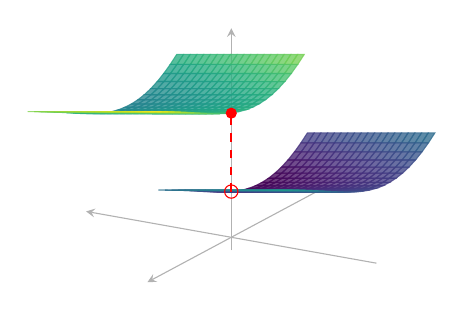
\begin{tikzpicture}
        \begin{axis}[
          view={210}{25},
          axis lines=center,
          xtick=\empty,
          ytick=\empty,
          ztick=\empty,
          xmin=-1.8, xmax=1.8,
          ymin=-1.8, ymax=1.8,
          zmin=-0.2, zmax=3.2,
          domain=-1.6:-0.02,
          y domain=-1.6:1.6,
          samples=20,
          samples y=24,
          width=7.4cm,
          height=6.2cm,
          colormap/viridis,
          shader=flat,
          draw=black!30,
        ]
          \addplot3[
            surf,
            opacity=0.78,
          ]
          {0.7 + 0.18*y^2 - 0.22*x + 0.22*sin(deg(1.4*y))};

          \addplot3[
            surf,
            opacity=0.78,
            domain=0.02:1.6,
          ]
          {1.9 + 0.18*y^2 - 0.22*x + 0.22*sin(deg(1.4*y))};

          \addplot3[
            dashed,
            thick,
            color=red,
          ]
          coordinates {
            (0,0,{0.7})
            (0,0,{1.9})
          };

          \addplot3[
            only marks,
            mark=o,
            mark size=2.4pt,
            color=red,
            fill=white,
          ]
          coordinates {(0,0,0.7)};

          \addplot3[
            only marks,
            mark=*,
            mark size=1.8pt,
            color=red,
          ]
          coordinates {(0,0,1.9)};
        \end{axis}
      \end{tikzpicture}
      \caption{A jump discontinuity across a curve.}
    \end{subfigure}
    \caption{Two typical discontinuities that can still occur in integrable functions: a removable hole and a jump discontinuity.}
  \end{figure}

  \begin{enumerate}
    \item Given that there is a subset $N$ in $B$ with volume $0$ over which $f$ is not defined, we can integrate over $B \setminus N$. In the one and two dimensional cases, 
    \[\int_{B \setminus N} f(x) dx \text{ and } \iint_{B\setminus N} f(x) dA\]
    are well-defined. Visually, this corresponds to a surface with a puncture over a set of measure zero. 
    \item The function is defined for all values in the region, but there is a jump in the value of the function. 
    Here the domain remains intact, but the graph splits into two sheets separated by a finite jump. 
  \end{enumerate}
  Informally, if we can visualize the Riemann sum converging to a well-defined area as the rectangles get thinner and thinner, then a discontinuous function is integrable. Indeed, all continuous functions (over a bounded set) are integrable since their Riemann sums are well defined. 

\subsection{Iterated Integrals} 

  The construction of the integral is one step, but we should know how to practically compute such an integral. We can do this by recursively ``reducing'' the dimension of the region of the integral until we can work with one dimension at which point we can use the univariate Riemann integral. This is informally known as \textit{Cavalieri's principle}, which states the following. 

	\begin{theorem}[Cavalieri's Principle]
		\begin{enumerate}
			\item Suppose two shapes in $\mathbb{R}^2$ are included between two parallel lines in that plane. If every line parallel to these two lines intersects both regions in line segments of equal length, then the two regions have equal areas. 

			\begin{figure}[H]
				\centering
				\begin{subfigure}[b]{0.48\textwidth}
					\centering
					\hspace{-3.7cm}
					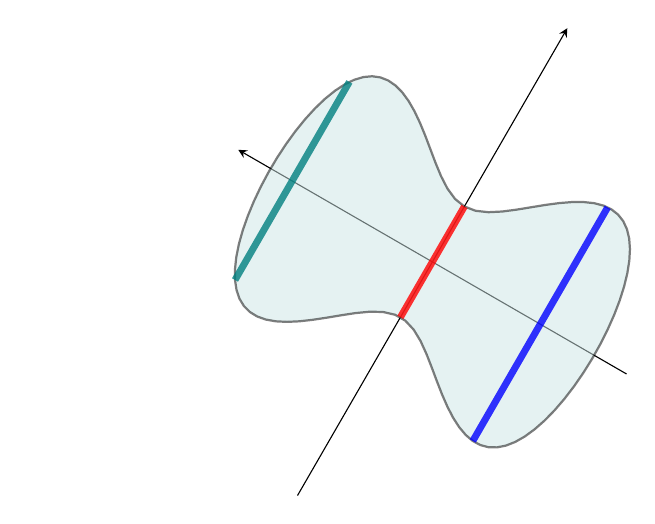
\begin{tikzpicture}
						\begin{axis}[
							axis lines=center,
							xmin=-2.0, xmax=2.0,
							ymin=-1.8, ymax=1.8,
							ticks=none,
							rotate around={60:(0,0)} 
						]
							
							% 2D region of the original shape
							\addplot[
								domain=0:360,
								samples=100,
								fill=teal!20,
								opacity=0.5,
								thick,
								draw=black
							] ({1.5 * cos(x) * sqrt(0.1 + 1.575 * sin(x)^2)}, {1.5 * sin(x)});

							% Cross section 1: The Waist (y = 0.0)
							\addplot[color=red, line width=2.5pt, opacity=0.8] coordinates {
								(-0.4743, 0)
								(0.4743, 0)
							};
							
							% Cross section 2: The Lobe Bulge (y = -1.0)
							\addplot[color=blue, line width=2.5pt, opacity=0.8] coordinates {
								(-1.0, -1.0)
								(1.0, -1.0)
							};

							% Cross section 3: Near the Tip (y = 1.3)
							\addplot[color=teal, line width=2.5pt, opacity=0.8] coordinates {
								(-0.8476, 1.3)
								(0.8476, 1.3)
							};
						\end{axis}
					\end{tikzpicture}
					\caption{Original region in $\mathbb{R}^2$}
				\end{subfigure}
				\hfill 
				\begin{subfigure}[b]{0.48\textwidth}
					\centering
					\hspace{-4.2cm}
					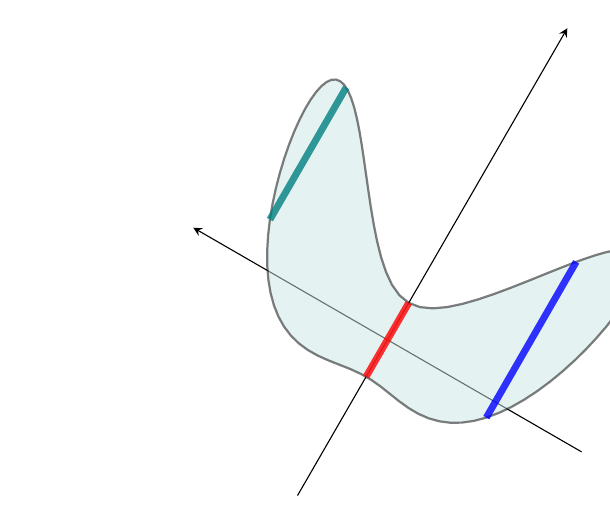
\begin{tikzpicture}
						\begin{axis}[
							axis lines=center,
							xmin=-2.0, xmax=4.0, % Expanded right side to fit the quadratic shift
							ymin=-1.8, ymax=1.8,
							ticks=none,
							rotate around={60:(0,0)} 
						]
							
							% 2D region of the quadratically sheared shape
							\addplot[
								domain=0:360,
								samples=100,
								fill=teal!20,
								opacity=0.5,
								thick,
								draw=black
							] ({1.5 * cos(x) * sqrt(0.1 + 1.575 * sin(x)^2) + 0.8 * (1.5 * sin(x))^2}, {1.5 * sin(x)});

							% Cross section 1: The Waist (y = 0.0)
							% Shift = 0.8 * (0)^2 = 0
							\addplot[color=red, line width=2.5pt, opacity=0.8] coordinates {
								(-0.4743 + 0, 0)
								(0.4743 + 0, 0)
							};
							
							% Cross section 2: The Lobe Bulge (y = -1.0)
							% Shift = 0.8 * (-1.0)^2 = 0.8
							\addplot[color=blue, line width=2.5pt, opacity=0.8] coordinates {
								(-1.0 + 0.8, -1.0)
								(1.0 + 0.8, -1.0)
							};

							% Cross section 3: Near the Tip (y = 1.3)
							% Shift = 0.8 * (1.3)^2 = 1.352
							\addplot[color=teal, line width=2.5pt, opacity=0.8] coordinates {
								(-0.8476 + 1.352, 1.3)
								(0.8476 + 1.352, 1.3)
							};
						\end{axis}
					\end{tikzpicture}
					\caption{Sheared region preserving 1D cross-sections}
				\end{subfigure}
				\caption{By Cavalieri's Principle in 2D, the area of the region is preserved because every 1D horizontal cross-section remains identical in length, despite the parabolic horizontal shear.}
				\label{fig:cavalieri_2d}
			\end{figure}

			\item Suppose two bodies in $\mathbb{R}^3$ are included between two parallel planes. If every plane parallel to these two planes intersects both regions in cross-sections of equal area, then the two regions have equal volumes.

			\begin{figure}[H]
				\centering
				\begin{subfigure}[b]{0.48\textwidth}
					\centering
					\hspace{-5.2cm}
					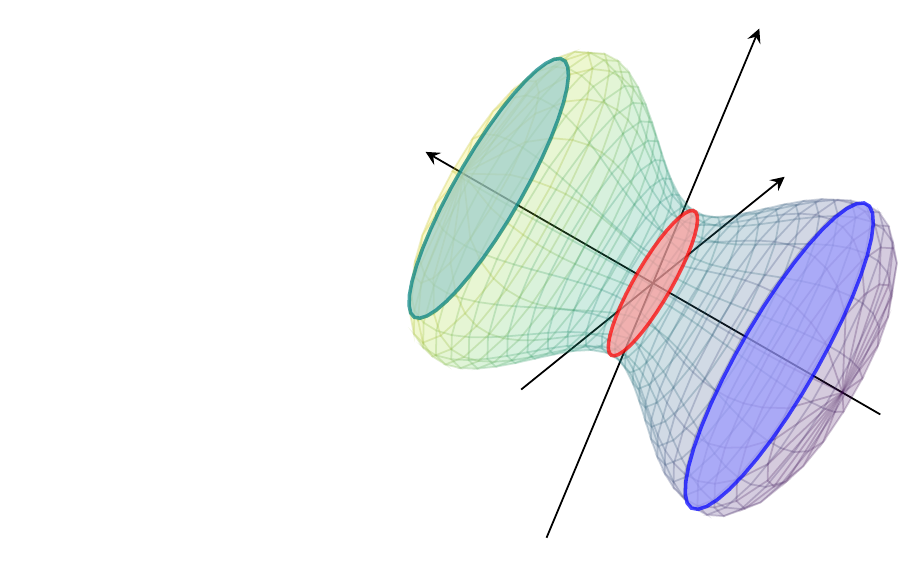
\begin{tikzpicture}[scale=1.6]
						\begin{axis}[
							view={60}{15},
							axis lines=center,
							xmin=-1.8, xmax=1.8,
							ymin=-1.8, ymax=1.8,
							zmin=-1.8, zmax=1.8,
							ticks=none,
							% Tilts the entire 3D plot space by 30 degrees around the origin
							rotate around={60:(0,0,0)} 
						]
							
							% Faint context shell of the peanut
							\addplot3[
								surf,
								domain=-1.5:1.5,
								domain y=0:360,
								samples=30,
								samples y=20,
								z buffer=sort,
								colormap/viridis,
								opacity=0.12, 
								shader=faceted
							] (
								{sqrt((2.25 - x^2) * (0.1 + 0.7 * x^2)) * cos(y)},
								{sqrt((2.25 - x^2) * (0.1 + 0.7 * x^2)) * sin(y)},
								{x}
							);

							% Cross section 1: The Waist (z = 0.0)
							\addplot3[
								fill=red!40,
								draw=red,
								thick,
								opacity=0.7,
								domain=0:360,
								samples=40
							] (
								{0.4743 * cos(x)},
								{0.4743 * sin(x)},
								{0}
							);
							
							% Cross section 2: The Lobe Bulge (z = 1.0)
							\addplot3[
								fill=blue!40,
								draw=blue,
								thick,
								opacity=0.7,
								domain=0:360,
								samples=40
							] (
								{1.0 * cos(x)},
								{1.0 * sin(x)},
								{-1.0}
							);

							% Cross section 3: Near the Tip (z = 1.3)
							\addplot3[
								fill=teal!40,
								draw=teal,
								thick,
								opacity=0.7,
								domain=0:360,
								samples=40
							] (
								{0.8476 * cos(x)},
								{0.8476 * sin(x)},
								{1.3}
							);
						\end{axis}
					\end{tikzpicture}
					\caption{}
				\end{subfigure}
				\hfill 
				\begin{subfigure}[b]{0.48\textwidth}
					\centering
					\hspace{-5.2cm}
					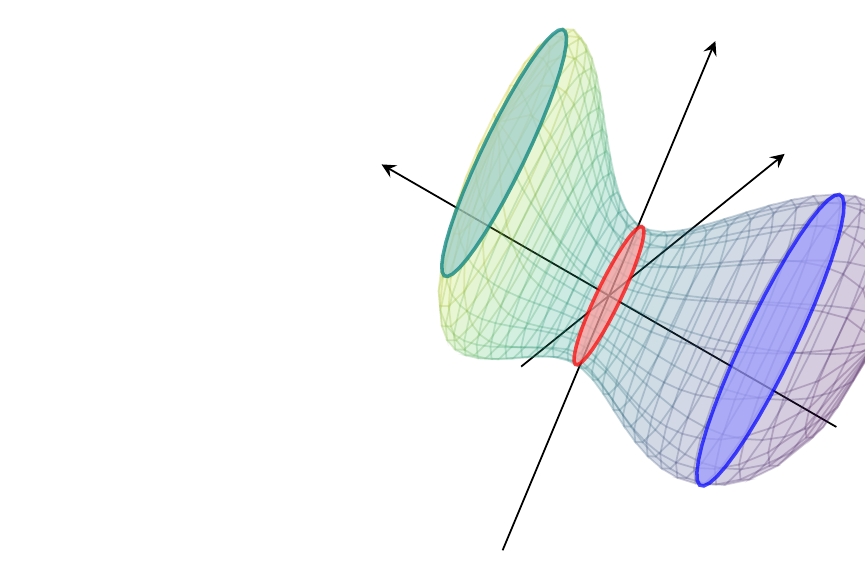
\begin{tikzpicture}[scale=1.6]
						\begin{axis}[
							view={60}{15},
							axis lines=center,
							xmin=-2.0, xmax=4.0, % Expanded right side to fit the quadratic shift
							ymin=-1.8, ymax=1.8,
							zmin=-1.8, zmax=1.8,
							ticks=none,
							% Tilts the entire 3D plot space by 30 degrees around the origin
							rotate around={60:(0,0,0)} 
						]
							
							% Faint context shell of the quadratically sheared peanut
							\addplot3[
								surf,
								domain=-1.5:1.5,
								domain y=0:360,
								samples=30,
								samples y=20,
								z buffer=sort,
								colormap/viridis,
								opacity=0.12, 
								shader=faceted
							] (
								{sqrt((2.25 - x^2) * (0.1 + 0.7 * x^2)) * cos(y) + 0.8 * x^2}, % Applied the 0.8z^2 shear
								{sqrt((2.25 - x^2) * (0.1 + 0.7 * x^2)) * sin(y)},
								{x}
							);

							% Cross section 1: The Waist (z = 0.0)
							% Shift = 0.8 * (0)^2 = 0
							\addplot3[
								fill=red!40,
								draw=red,
								thick,
								opacity=0.7,
								domain=0:360,
								samples=40
							] (
								{0.4743 * cos(x) + 0},
								{0.4743 * sin(x)},
								{0}
							);
							
							% Cross section 2: The Lobe Bulge (z = -1.0)
							% Shift = 0.8 * (-1.0)^2 = 0.8
							\addplot3[
								fill=blue!40,
								draw=blue,
								thick,
								opacity=0.7,
								domain=0:360,
								samples=40
							] (
								{1.0 * cos(x) + 0.8},
								{1.0 * sin(x)},
								{-1.0}
							);

							% Cross section 3: Near the Tip (z = 1.3)
							% Shift = 0.8 * (1.3)^2 = 1.352
							\addplot3[
								fill=teal!40,
								draw=teal,
								thick,
								opacity=0.7,
								domain=0:360,
								samples=40
							] (
								{0.8476 * cos(x) + 1.352},
								{0.8476 * sin(x)},
								{1.3}
							);
						\end{axis}
					\end{tikzpicture}
					\caption{}
				\end{subfigure}
				\caption{Even though the two are different solids in $\mathbb{R}^3$, the cross sections are the same. Therefore, Cavalieri's principle states that the volumes of the two solids must be equal. }
				\label{fig:cavalieri}
			\end{figure}
		\end{enumerate}
	\end{theorem}


	In the case when $S$ is a box in $\mathbb{R}^n$, Fubini's theorem states that whether we cut $S$ up along the $x_1$-axis, $x_2$-axis, ..., or the $x_n$-axis, the symmetry in volume is always preserved. This theorem is really just a specific case of this general symmetry in volume. 

  \begin{theorem}[Euler-Fubini Theorem]
    Given a function $f: \mathbb{R}^n \longrightarrow \mathbb{R}$, let $B \coloneqq \prod_{i=1}^n [\alpha_i, \beta_i]$ and let $p$ be any permutation of the elements $\{x_1, x_2, \ldots, x_n\}$. Then 
    \begin{equation}
        \int_B f \, d V = \int_{\alpha_n}^{\beta_n} \ldots \int_{\alpha_1}^{\beta_1} f \, d x_1 \ldots d x_n = \int_{p(\alpha_n)}^{p(\beta_n)} \ldots \int_{p(\alpha_1)}^{p(\beta_1)} f \, d p(x_1) \ldots d p(x_n) 
    \end{equation}
  \end{theorem}
	\begin{proof}

	\end{proof}

  In the two dimensional case, we have
  \begin{equation}
		\iint_B f \, d A = \int_c^d \int_a^b f(x, y) \, d x \, d y = \int_a^b \int_c^d f(x, y) \, d y \, d x 
  \end{equation}

  \begin{figure}[H]
    \centering
    \begin{subfigure}[b]{0.48\textwidth}
      \centering
			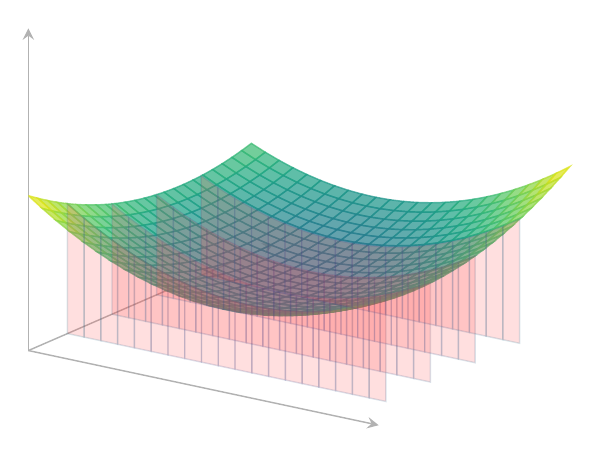
\begin{tikzpicture}[scale=1.3]
        \begin{axis}[
          view={35}{22},
          axis lines=center,
          xtick=\empty,
          ytick=\empty,
          ztick=\empty,
          xmin=0, xmax=2.2,
          ymin=0, ymax=2.2,
          zmin=0, zmax=2.6,
          domain=0:2,
          y domain=0:2,
          samples=24,
          samples y=24,
          width=7.4cm,
          height=6.5cm,
          colormap/viridis,
          shader=flat,
          draw=black!30,
        ]
          \addplot3[
            surf,
            opacity=0.72,
          ]
          {0.45 + 0.38*(x-1)^2 + 0.24*(y-1)^2 + 0.18*(x-1)*(y-1)};

          \foreach \yy in {0.35,0.75,1.15,1.55} {
            \addplot3[
              surf,
              opacity=0.18,
              draw=none,
              fill=red!70,
              domain=0:2,
              y domain=0:1,
              samples=20,
              samples y=2,
            ]
            ({x}, {\yy}, {y*(0.45 + 0.38*(x-1)^2 + 0.24*(\yy-1)^2 + 0.18*(x-1)*(\yy-1))});

          }
        \end{axis}
      \end{tikzpicture}
      \caption{Slicing at fixed values of $y$.}
    \end{subfigure}
    \hfill
    \begin{subfigure}[b]{0.48\textwidth}
      \centering
			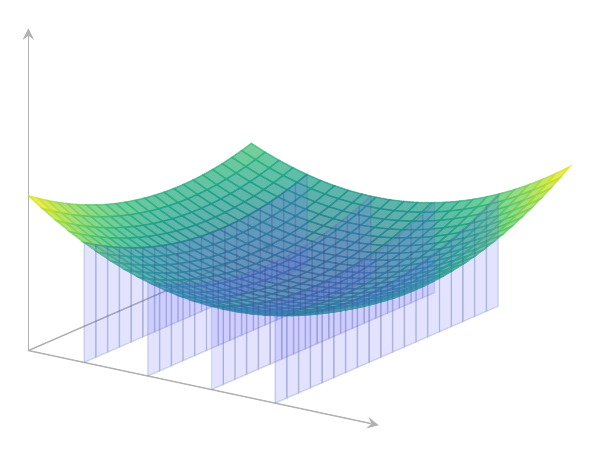
\begin{tikzpicture}[scale=1.3]
        \begin{axis}[
          view={35}{22},
          axis lines=center,
          xtick=\empty,
          ytick=\empty,
          ztick=\empty,
          xmin=0, xmax=2.2,
          ymin=0, ymax=2.2,
          zmin=0, zmax=2.6,
          domain=0:2,
          y domain=0:2,
          samples=24,
          samples y=24,
          width=7.4cm,
          height=6.5cm,
          colormap/viridis,
          shader=flat,
          draw=black!30,
        ]
          \addplot3[
            surf,
            opacity=0.72,
          ]
          {0.45 + 0.38*(x-1)^2 + 0.24*(y-1)^2 + 0.18*(x-1)*(y-1)};

          \foreach \xx in {0.35,0.75,1.15,1.55} {
            \addplot3[
              surf,
              opacity=0.18,
              draw=none,
              fill=blue!60,
              domain=0:1,
              y domain=0:2,
              samples=2,
              samples y=20,
            ]
            ({\xx}, {y}, {x*(0.45 + 0.38*(\xx-1)^2 + 0.24*(y-1)^2 + 0.18*(\xx-1)*(y-1))});

          }
        \end{axis}
      \end{tikzpicture}
      \caption{Slicing at fixed values of $x$.}
    \end{subfigure}
  \end{figure}

  and in the three dimensional case, we can use any of the 6 permutations. Computation of these integrals is simple. You do the innermost integral first with respect to the corresponding variable, while treating the rest of the variables constant. Evaluating each integral outputs a formula for a higher dimensional cross section of the solid $S$. It is clear that computing iterated integrals is really just doing Cavalieri's principle repeatedly. 

  \begin{example}[Double Integral over a Rectangle: Easy]
    Let 
    \[D = [0,1] \times [0,2]\]
    and consider the function $f(x,y) = x + 2y$. Then 
    \begin{center}
    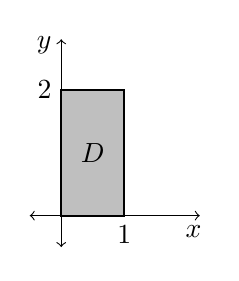
\begin{tikzpicture}[scale=0.8]
      \draw[<->] (-0.5,0)--(2.2,0);
      \draw[<->] (0,-0.5)--(0,2.8);
      \fill[lightgray] (0,0) rectangle (1,2);
      \draw[thick] (0,0) rectangle (1,2);
      \node at (0.5,1) {$D$};
      \node[below] at (1,0) {$1$};
      \node[left] at (0,2) {$2$};
      \node[below] at (2.1,0) {$x$};
      \node[left] at (0,2.7) {$y$};
    \end{tikzpicture}
    \end{center}
    Since $D$ is a rectangle, we may write
    \begin{align*}
      \iint_D (x+2y)\,dA
      &= \int_0^2 \int_0^1 (x+2y)\,dx\,dy \\
      &= \int_0^2 \left[ \frac{x^2}{2} + 2yx \right]_{x=0}^{x=1} dy \\
      &= \int_0^2 \left( \frac{1}{2} + 2y \right) dy \\
      &= \left[ \frac{y}{2} + y^2 \right]_{y=0}^{y=2} \\
      &= 1 + 4 = 5.
    \end{align*}
    Therefore,
    \[\iint_D (x+2y)\,dA = 5.\]
  \end{example}

  \begin{example}[Double Integral over a Rectangle: Hard]
    Let 
    \[D = [1,2] \times [0,\ln 2]\]
    and let $f(x,y) = x e^y$. Then 
    \begin{center}
    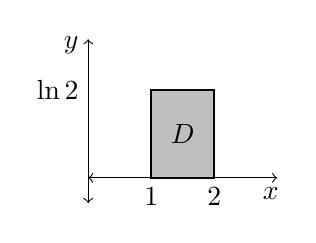
\begin{tikzpicture}[scale=0.8]
      \draw[<->] (0,0)--(3,0);
      \draw[<->] (0,-0.4)--(0,2.2);
      \fill[lightgray] (1,0) rectangle (2,1.4);
      \draw[thick] (1,0) rectangle (2,1.4);
      \node at (1.5,0.7) {$D$};
      \node[below] at (1,0) {$1$};
      \node[below] at (2,0) {$2$};
      \node[left] at (0,1.4) {$\ln 2$};
      \node[below] at (2.9,0) {$x$};
      \node[left] at (0,2.1) {$y$};
    \end{tikzpicture}
    \end{center}
    Again, the region is rectangular, so
    \begin{align*}
      \iint_D x e^y\,dA
      &= \int_0^{\ln 2} \int_1^2 x e^y\,dx\,dy \\
      &= \int_0^{\ln 2} e^y \left[ \frac{x^2}{2} \right]_{x=1}^{x=2} dy \\
      &= \int_0^{\ln 2} \frac{3}{2} e^y\,dy \\
      &= \frac{3}{2} \left[ e^y \right]_{y=0}^{y=\ln 2} \\
      &= \frac{3}{2}(2-1) = \frac{3}{2}.
    \end{align*}
    Hence,
    \[\iint_D x e^y\,dA = \frac{3}{2}.\]
  \end{example}

  \begin{example}[Triple Integral over a Box: Easy]
    Let 
    \[B = [0,1] \times [0,2] \times [0,1]\]
    and let $f(x,y,z) = x+y+z$. Then 
    \begin{center}
    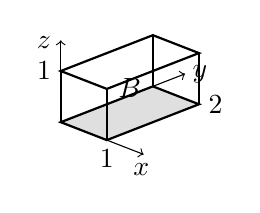
\begin{tikzpicture}[scale=0.65, x={(0.9cm,-0.35cm)}, y={(0.9cm,0.35cm)}, z={(0cm,1cm)}]
      \fill[lightgray, opacity=0.5] (0,0,0) -- (1,0,0) -- (1,2,0) -- (0,2,0) -- cycle;
      \draw[->] (0,0,0)--(1.8,0,0);
      \draw[->] (0,0,0)--(0,2.7,0);
      \draw[->] (0,0,0)--(0,0,1.6);
      \draw[thick] (0,0,0)--(1,0,0)--(1,2,0)--(0,2,0)--cycle;
      \draw[thick] (0,0,1)--(1,0,1)--(1,2,1)--(0,2,1)--cycle;
      \draw[thick] (0,0,0)--(0,0,1);
      \draw[thick] (1,0,0)--(1,0,1);
      \draw[thick] (1,2,0)--(1,2,1);
      \draw[thick] (0,2,0)--(0,2,1);
      \node at (0.5,1,0.5) {$B$};
      \node[below] at (1,0,0) {$1$};
      \node[right] at (1,2,0) {$2$};
      \node[left] at (0,0,1) {$1$};
      \node[below] at (1.75,0,0) {$x$};
      \node[right] at (0,2.65,0) {$y$};
      \node[left] at (0,0,1.55) {$z$};
    \end{tikzpicture}
    \end{center}
    Using the order $dz\,dy\,dx$, we get
    \begin{align*}
      \iiint_B (x+y+z)\,dV
      &= \int_0^1 \int_0^2 \int_0^1 (x+y+z)\,dz\,dy\,dx \\
      &= \int_0^1 \int_0^2 \left[ (x+y)z + \frac{z^2}{2} \right]_{z=0}^{z=1} dy\,dx \\
      &= \int_0^1 \int_0^2 \left( x+y+\frac{1}{2} \right) dy\,dx \\
      &= \int_0^1 \left[ xy + \frac{y^2}{2} + \frac{y}{2} \right]_{y=0}^{y=2} dx \\
      &= \int_0^1 (2x+3)\,dx \\
      &= \left[ x^2 + 3x \right]_{x=0}^{x=1} \\
      &= 1+3 = 4.
    \end{align*}
    Therefore,
    \[\iiint_B (x+y+z)\,dV = 4.\]
  \end{example}

  \begin{example}[Triple Integral over a Box: Hard]
    Let 
    \[B = [1,2] \times [0,\ln 2] \times [0,1]\]
    and let $f(x,y,z) = x e^y (1+z^2)$. Then 
    \begin{center}
    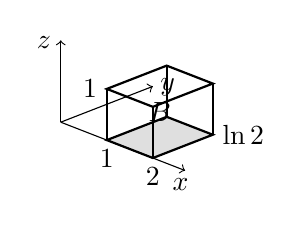
\begin{tikzpicture}[scale=0.65, x={(0.9cm,-0.35cm)}, y={(0.9cm,0.35cm)}, z={(0cm,1cm)}]
      \fill[lightgray, opacity=0.5] (1,0,0) -- (2,0,0) -- (2,1.3,0) -- (1,1.3,0) -- cycle;
      \draw[->] (0,0,0)--(2.7,0,0);
      \draw[->] (0,0,0)--(0,2,0);
      \draw[->] (0,0,0)--(0,0,1.6);
      \draw[thick] (1,0,0)--(2,0,0)--(2,1.3,0)--(1,1.3,0)--cycle;
      \draw[thick] (1,0,1)--(2,0,1)--(2,1.3,1)--(1,1.3,1)--cycle;
      \draw[thick] (1,0,0)--(1,0,1);
      \draw[thick] (2,0,0)--(2,0,1);
      \draw[thick] (2,1.3,0)--(2,1.3,1);
      \draw[thick] (1,1.3,0)--(1,1.3,1);
      \node at (1.5,0.65,0.5) {$B$};
      \node[below] at (1,0,0) {$1$};
      \node[below] at (2,0,0) {$2$};
      \node[right] at (2,1.3,0) {$\ln 2$};
      \node[left] at (1,0,1) {$1$};
      \node[below] at (2.6,0,0) {$x$};
      \node[right] at (0,1.95,0) {$y$};
      \node[left] at (0,0,1.55) {$z$};
    \end{tikzpicture}
    \end{center}
    With the order $dz\,dy\,dx$, we obtain
    \begin{align*}
      \iiint_B x e^y (1+z^2)\,dV
      &= \int_1^2 \int_0^{\ln 2} \int_0^1 x e^y (1+z^2)\,dz\,dy\,dx \\
      &= \int_1^2 \int_0^{\ln 2} x e^y \left[ z + \frac{z^3}{3} \right]_{z=0}^{z=1} dy\,dx \\
      &= \int_1^2 \int_0^{\ln 2} \frac{4}{3} x e^y\,dy\,dx \\
      &= \int_1^2 \frac{4}{3} x \left[ e^y \right]_{y=0}^{y=\ln 2} dx \\
      &= \int_1^2 \frac{4}{3}x\,dx \\
      &= \frac{4}{3} \left[ \frac{x^2}{2} \right]_{x=1}^{x=2} \\
      &= \frac{4}{3}\cdot \frac{3}{2} = 2.
    \end{align*}
    Hence,
    \[\iiint_B x e^y (1+z^2)\,dV = 2.\]
  \end{example}

\subsection{Integration over Regions between Curves} 

  \begin{definition}[Simple Regions w.r.t. a Variable]
    A bounded region $D$ in $\mathbb{R}^n$ is said to be $x_i$-simple if it is bounded by the graphs of two continuous functions $u_1, u_2: \mathbb{R}^{n-1} \longrightarrow \mathbb{R}$ of the variables 
    \[x_1, x_2, ..., x_{i-1}, x_{i+1}, ..., x_n\]
    That is, $D$ can be expressed in the form 
    \[\{ x \in \mathbb{R}^n \; | \; u_1 (x_1,..., x_{i-1}, x_{i+1}, ... , x_n) \leq x_i \leq u_2 (x_1, ..., x_{i-1}, x_{i+1}, ..., x_n)\}\]
    If a region is simple in all of its variables, it is simply called \textit{simple}. Note that $n$-dimensional boxes are simple regions. 
  \end{definition}

  \begin{example}
    In $\mathbb{R}^2$, the region on the left graph is an $y$-simple region and the region on the right is a $x$-simple region. 
    \begin{center}
    \begin{tikzpicture}[scale=0.8]
      \draw[<->] (-1,0)--(5,0);
      \draw[<->] (0,-1)--(0,5);
      \draw[<->] (6,0)--(12,0);
      \draw[<->] (7,-1)--(7,5);
      \draw plot [smooth] coordinates {(0.6, 1.2) (1,1) (2,1.4) (3,1.3) (4,1.5) (4.3,1.7)};
      \draw plot [smooth] coordinates {(0.6, 3.9) (1,4.1) (2,4) (3,4.3) (4,4.2) (4.3,4.1)};
      \draw[dashed] (0.6,1.2)--(0.6,3.9);
      \draw[dashed] (4.3,1.7)--(4.3,4.1);
      \draw plot [smooth] coordinates {(8.2,0.6) (8,1) (8.4,2) (8.3,3) (8.5,4) (8.7,4.3)};
      \draw plot [smooth] coordinates {(10.9,0.6) (11.1,1) (11,2) (11.3,3) (11.2,4) (11.1,4.3)};
      \draw[dashed] (8.2,0.6)--(10.9,0.6);
      \draw[dashed] (8.7,4.3)--(11.1,4.3);
      \node[below] at (4.8,0) {$x$};
      \node[below] at (11.8,0) {$x$};
      \node[left] at (0,4.8) {$y$};
      \node[left] at (7,4.8) {$y$};
      \node[above] at (3,4.2) {$u_1$};
      \node[above] at (3,1.3) {$u_2$};
      \node[left] at (8.3, 3) {$v_1$};
      \node[right] at (11.3, 3) {$v_2$};
      \draw[fill] (0.6,0) circle (0.05);
      \node[below] at (0.6,0) {$a$};
      \draw[fill] (4.3,0) circle (0.05);
      \node[below left] at (4.3,0) {$b$};
      \draw[fill] (7,0.6) circle (0.05);
      \draw[fill] (7,4.3) circle (0.05);
      \node[left] at (7,0.6) {$c$};
      \node[left] at (7,4.3) {$d$};
    \end{tikzpicture}
    \end{center}
  \end{example}

  We now describe the method of calculating double integrals over elementary regions. 

	\begin{theorem}[Iterated Integrals over Simple Regions]
		The double integral over a $y$-simple region $D$ bounded by functions $u_1$ and $u_2$ in $\mathbb{R}^2$ and the $x$-values $a$ and $b$ (as shown in the left graph of example 2.1) is
		\begin{equation}
			\iint_D f(x, y) = \int_a^b \int_{u_2 (x)}^{u_1 (x)} f(x, y) \, dy \, dx
		\end{equation}
		The double integral over an $x$-simple region $D$ bounded by functions $v_1$ and $v_2$ in $\mathbb{R}^2$ and the $y$-values $c$ and $d$ (shown in the right of graph of example 2.1) is 
		\begin{equation}
			\iint_D f(x, y) = \int_c^d \int_{v_2 (y)}^{v_1 (y)} f(x, y) \, dx \, dy
		\end{equation}
  \end{theorem}

	\begin{example}[Unit Disk]
		Integrating $f(x, y)$ over the unit disk would have the form
		\begin{equation}
			\int_{-1}^1 \int_{-\sqrt{1-x^2}}^{\sqrt{1-x^2}} f(x,y) \, dy\, dx \text{ or } \int_{-1}^1 \int_{-\sqrt{1-y^2}}^{\sqrt{1-y^2}} f(x,y) \, dx\, dy 
		\end{equation}
		Note that the unit disk is both $x$ and $y$ simple. 
  \end{example}

  \begin{example}[Double Integral over a Non-Rectangular Region: Easy]
    Consider the triangular region
    \[D = \{(x,y) \in \mathbb{R}^2 \mid 0 \leq x \leq 1,\; x \leq y \leq 1\}\]
    and let $f(x,y) = x+y$. Then 
    \begin{center}
    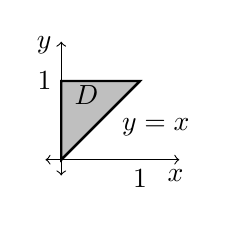
\begin{tikzpicture}[scale=1]
      \draw[<->] (-0.2,0)--(1.5,0);
      \draw[<->] (0,-0.2)--(0,1.5);
      \fill[lightgray] (0,0) -- (0,1) -- (1,1) -- cycle;
      \draw[thick] (0,0) -- (0,1) -- (1,1) -- cycle;
      \draw[thick] (0,0) -- (1,1);
      \node at (0.32,0.82) {$D$};
      \node[below] at (1,0) {$1$};
      \node[left] at (0,1) {$1$};
      \node[below] at (1.45,0) {$x$};
      \node[left] at (0,1.45) {$y$};
      \node[below right] at (0.65,0.65) {$y=x$};
    \end{tikzpicture}
    \end{center}
    Since $D$ is $y$-simple,
    \begin{align*}
      \iint_D (x+y)\,dA
      &= \int_0^1 \int_x^1 (x+y)\,dy\,dx \\
      &= \int_0^1 \left[ xy + \frac{y^2}{2} \right]_{y=x}^{y=1} dx \\
      &= \int_0^1 \left( x+\frac{1}{2} - x^2 - \frac{x^2}{2} \right) dx \\
      &= \int_0^1 \left( x+\frac{1}{2} - \frac{3x^2}{2} \right) dx \\
      &= \left[ \frac{x^2}{2} + \frac{x}{2} - \frac{x^3}{2} \right]_{x=0}^{x=1} \\
      &= \frac{1}{2}.
    \end{align*}
    Therefore,
    \[\iint_D (x+y)\,dA = \frac{1}{2}.\]
  \end{example}

  \begin{example}[Double Integral over a Non-Rectangular Region: Hard]
    Let 
    \[D = \{(x,y) \in \mathbb{R}^2 \mid 1 \leq x \leq 2,\; 0 \leq y \leq \ln x\}\]
    and let $f(x,y) = y e^y$. Then 
    \begin{center}
    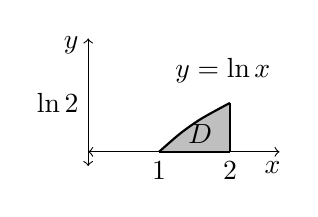
\begin{tikzpicture}[scale=0.9]
      \draw[<->] (0,0)--(2.7,0);
      \draw[<->] (0,-0.2)--(0,1.6);
      \fill[lightgray] (1,0) -- plot[smooth] coordinates {(1,0) (1.3,0.26) (1.6,0.47) (2,0.69)} -- (2,0) -- cycle;
      \draw[thick] (1,0) -- (2,0);
      \draw[thick] (1,0) -- (1,0);
      \draw[thick] plot[smooth] coordinates {(1,0) (1.3,0.26) (1.6,0.47) (2,0.69)};
      \draw[thick] (2,0) -- (2,0.69);
      \node at (1.58,0.25) {$D$};
      \node[below] at (1,0) {$1$};
      \node[below] at (2,0) {$2$};
      \node[left] at (0,0.69) {$\ln 2$};
      \node[below] at (2.6,0) {$x$};
      \node[left] at (0,1.5) {$y$};
      \node[above] at (1.9,0.83) {$y=\ln x$};
    \end{tikzpicture}
    \end{center}
    This region is not a rectangle because its upper boundary depends on $x$. We compute
    \begin{align*}
      \iint_D y e^y\,dA
      &= \int_1^2 \int_0^{\ln x} y e^y\,dy\,dx \\
      &= \int_1^2 \left[ (y-1)e^y \right]_{y=0}^{y=\ln x} dx \\
      &= \int_1^2 \left( x \ln x - x + 1 \right) dx \\
      &= \left[ \frac{x^2}{2}\ln x - \frac{x^2}{4} - \frac{x^2}{2} + x \right]_{x=1}^{x=2} \\
      &= \left( 2\ln 2 - 1 \right) - \frac{1}{4} \\
      &= 2\ln 2 - \frac{5}{4}.
    \end{align*}
    Thus,
    \[\iint_D y e^y\,dA = 2\ln 2 - \frac{5}{4}.\]
  \end{example}

  \begin{example}[Triple Integral over a Non-Rectangular Region: Easy]
    Consider the solid
    \[S = \{(x,y,z) \in \mathbb{R}^3 \mid 0 \leq x \leq 1,\; 0 \leq y \leq 1-x,\; 0 \leq z \leq 2\}\]
    and let $f(x,y,z) = x+y+z$. Then 
    \begin{center}
    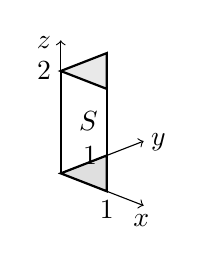
\begin{tikzpicture}[scale=0.65, x={(0.9cm,-0.35cm)}, y={(0.9cm,0.35cm)}, z={(0cm,1cm)}]
      \fill[lightgray, opacity=0.5] (0,0,0) -- (1,0,0) -- (0,1,0) -- cycle;
      \fill[lightgray, opacity=0.35] (0,0,2) -- (1,0,2) -- (0,1,2) -- cycle;
      \draw[->] (0,0,0)--(1.8,0,0);
      \draw[->] (0,0,0)--(0,1.8,0);
      \draw[->] (0,0,0)--(0,0,2.6);
      \draw[thick] (0,0,0)--(1,0,0)--(0,1,0)--cycle;
      \draw[thick] (0,0,2)--(1,0,2)--(0,1,2)--cycle;
      \draw[thick] (0,0,0)--(0,0,2);
      \draw[thick] (1,0,0)--(1,0,2);
      \draw[thick] (0,1,0)--(0,1,2);
      \node at (0.28,0.32,1) {$S$};
      \node[below] at (1,0,0) {$1$};
      \node[left] at (0,1,0) {$1$};
      \node[left] at (0,0,2) {$2$};
      \node[below] at (1.75,0,0) {$x$};
      \node[right] at (0,1.75,0) {$y$};
      \node[left] at (0,0,2.55) {$z$};
    \end{tikzpicture}
    \end{center}
    The base in the $xy$-plane is triangular, so the bounds are not independent. We compute
    \begin{align*}
      \iiint_S (x+y+z)\,dV
      &= \int_0^1 \int_0^{1-x} \int_0^2 (x+y+z)\,dz\,dy\,dx \\
      &= \int_0^1 \int_0^{1-x} \left[ (x+y)z + \frac{z^2}{2} \right]_{z=0}^{z=2} dy\,dx \\
      &= \int_0^1 \int_0^{1-x} (2x+2y+2)\,dy\,dx \\
      &= \int_0^1 \left[ 2xy + y^2 + 2y \right]_{y=0}^{y=1-x} dx \\
      &= \int_0^1 \left( 3 - 2x - x^2 \right) dx \\
      &= \left[ 3x - x^2 - \frac{x^3}{3} \right]_{x=0}^{x=1} \\
      &= 3-1-\frac{1}{3} = \frac{5}{3}.
    \end{align*}
    Hence,
    \[\iiint_S (x+y+z)\,dV = \frac{5}{3}.\]
  \end{example}

  \begin{example}[Triple Integral over a Non-Rectangular Region: Hard]
    Let 
    \[S = \{(x,y,z) \in \mathbb{R}^3 \mid 1 \leq x \leq 2,\; 0 \leq y \leq \ln x,\; 0 \leq z \leq y\}\]
    and let $f(x,y,z) = e^y(1+z)$. Then 
    \begin{center}
    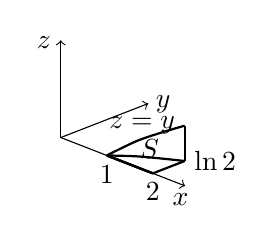
\begin{tikzpicture}[scale=0.65, x={(0.9cm,-0.35cm)}, y={(0.9cm,0.35cm)}, z={(0cm,1cm)}]
      \draw[->] (0,0,0)--(2.7,0,0);
      \draw[->] (0,0,0)--(0,1.9,0);
      \draw[->] (0,0,0)--(0,0,1.9);
      \draw[thick] (1,0,0)--(2,0,0);
      \draw[thick] plot[smooth] coordinates {(1,0,0) (1.35,0.3,0) (1.7,0.52,0) (2,0.69,0)};
      \draw[thick] plot[smooth] coordinates {(1,0,0) (1.35,0.3,0.3) (1.7,0.52,0.52) (2,0.69,0.69)};
      \draw[thick] (2,0,0)--(2,0.69,0);
      \draw[thick] (2,0,0)--(2,0,0);
      \draw[thick] (2,0.69,0)--(2,0.69,0.69);
      \draw[thick] (1,0,0)--(1,0,0);
      \foreach \t/\yy in {1/0,2/0.69} {
        \draw[dashed] (\t,\yy,0)--(\t,\yy,\yy);
      }
      \draw[thick] (1,0,0) -- (2,0,0);
      \draw[thick] (1,0,0) -- (2,0,0);
      \node at (1.65,0.28,0.26) {$S$};
      \node[below] at (1,0,0) {$1$};
      \node[below] at (2,0,0) {$2$};
      \node[right] at (2,0.69,0) {$\ln 2$};
      \node[left] at (2,0.69,0.69) {$z=y$};
      \node[below] at (2.6,0,0) {$x$};
      \node[right] at (0,1.85,0) {$y$};
      \node[left] at (0,0,1.85) {$z$};
    \end{tikzpicture}
    \end{center}
    Here both the $y$- and $z$-bounds depend on earlier variables. Using the order $dz\,dy\,dx$,
    \begin{align*}
      \iiint_S e^y(1+z)\,dV
      &= \int_1^2 \int_0^{\ln x} \int_0^y e^y(1+z)\,dz\,dy\,dx \\
      &= \int_1^2 \int_0^{\ln x} e^y \left[ z + \frac{z^2}{2} \right]_{z=0}^{z=y} dy\,dx \\
      &= \int_1^2 \int_0^{\ln x} e^y \left( y + \frac{y^2}{2} \right) dy\,dx \\
      &= \int_1^2 \left[ \frac{y^2}{2} e^y \right]_{y=0}^{y=\ln x} dx \\
      &= \int_1^2 \frac{x(\ln x)^2}{2}\,dx \\
      &= \left[ \frac{x^2}{4}(\ln x)^2 - \frac{x^2}{4}\ln x + \frac{x^2}{8} \right]_{x=1}^{x=2} \\
      &= \left( (\ln 2)^2 - \ln 2 + \frac{1}{2} \right) - \frac{1}{8} \\
      &= (\ln 2)^2 - \ln 2 + \frac{3}{8}.
    \end{align*}
    Therefore,
    \[\iiint_S e^y(1+z)\,dV = (\ln 2)^2 - \ln 2 + \frac{3}{8}.\]
  \end{example}

\subsection{Change of Basis}

  Sometimes, integrating a region over a different basis would make the integral computation much more simpler. In this case, we may be able to transform more complicated regions into elementary regions. We first introduce a change of basis in 2 dimensions and then generalize it into higher dimensions. 
  
  Let $\mathbb{R}^2$ have the standard orthonomal basis $e_1, e_2$, commonly known as the $x, y$ basis. Now, let us construct new basis vectors of $\mathbb{R}^2$, denoted $f_1, f_2$ such that $f_1, f_2$ are functions of $e_1, e_2$. Since they are both bases that span $\mathbb{R}^2$, we can equally represent $e_1, e_2$ as functions of $f_1, f_2$. 
  \begin{align*}
      &e_1 = g(f_1, f_2)\\
      &e_2 = h(f_1, f_2) 
  \end{align*}
  Note that this change of basis does not necessarily have to be linear, as in the context of passive transformation in linear algebra. Then, every point $(x,y)$ in the $(e_1, e_2)$-basis can be rewritten as
  \begin{align*}
      (x, y) & = x e_1 + y e_2 \\
      & = x \, g(f_1, f_2) + y \, h(f_1, f_2) \\
      & = u f_1 + v f_2
  \end{align*}
  Note that it is customary to denote $x, y$ as the coefficients in the $e_1, e_2$ basis and $u, v$ as the coefficients in the new $f_1, f_2$ basis. This way, we can not only write $e_1$ and $e_2$ as functions of $f_1$ and $f_2$, but we can also write the coefficents $x, y$ as functions of the coeffiecents $u, v$! That is, 
  \begin{align*}
      & x = x(u, v) \\
      & y = y(u, v)
  \end{align*}
  which is really just a function 
  \[B: \mathbb{R}^2 \longrightarrow \mathbb{R}^2, \;\; B(u, v) = \begin{pmatrix} x(u, v) \\ y(u, v) \end{pmatrix}\]
  Notice that $B$ changes the $u, v$ coordinates to the $x, y$ coordinates, and $B^{-1}$ changes the $x, y$ coordinates to the $u, v$ coordinates. 
  \[B^{-1}: \mathbb{R}^2 \longrightarrow \mathbb{R}^2, \;\; B^{-1} (x, y) = \begin{pmatrix} u (x, y) \\ v (x, y) \end{pmatrix}\]
  Note that these coefficients actually change \textit{contravariantly}, that is, they change inversely with respect to how the basis vectors are changed. In vector calculus, it is conventional to represent a change of basis with functions that relate the coefficients $x, y$ with $u, v$, rather than the bases $f_1, f_2$ with $e_1, e_2$. 

  \begin{theorem}[Integration over Change of Bases in $\mathbb{R}^2$]
  Let $\mathbb{R}^2$ have the standard orthonomal basis $e_1, e_2$. Now, let us construct new basis vectors of $\mathbb{R}^2$, denoted $f_1, f_2$ such that the coefficients of the vectors in $\mathbb{R}^2$ are related by the change of basis function 
  \[B = \begin{pmatrix} x \\ y \end{pmatrix} \implies B(u, v) = \begin{pmatrix} x(u, v) \\ y(u, v) \end{pmatrix}\]
  Given region $D \subset \mathbb{R}^2$ and $S = B(D)$ is the region transformed by $B$, the integral of function $f(x, y)$ over region $D$ can be expressed as 
  \[\iint_D f(x, y) \, dA = \iint_S f \big( x(u, v), y(u, v) \big) \, \big| J B(u, v) \big| \, d \bar{A}\]
  where $\big| J B(u, v) \big|$ is the determinant of the Jacobian matrix of $B$. Expanding the Facobian determinant gives
  \[\big| J B(u, v) \big| = \frac{\partial x}{\partial u} \frac{\partial y}{\partial v} - \frac{\partial x}{\partial v} \frac{\partial y}{\partial u}\]
  \end{theorem}

  \begin{theorem}[Integration over Change of Bases in $\mathbb{R}^3$]
  Given that we have the change of basis function 
  \[B: \mathbb{R}^3 \longrightarrow \mathbb{R}^3, \;\;\; B(u, v, w) = \begin{pmatrix} x(u, v, w) \\ y(u, v, w) \\ z(u, v, w) \end{pmatrix}\]
  a region $D \in \mathbb{R}^3$ and $S = B(D)$, the region transformed by $B$, the integral of $f(x, y, z)$ over region $D$ can be expressed as 
  \[\iiint_D f(x, y, z)\, dV = \iiint_S f\big( x(u, v, w), y(u, v ,w), z(u, v, w) \big) \big| J B (u, v, w)\big| \, d \bar{V}\]
  where $\big| J B (u, v, w)\big|$ is the Jacobian determinant of $B$. 
  \end{theorem}

  \begin{example}
  Given a real-valued function $f$ defined over the region $D \subset \mathbb{R}^2$, we can perform a change of basis of the $x, y$ coordinates into polar ones within a new region $S$. The change of basis 
  \begin{align*}
      & x = r \cos{\theta} \\
      & y = r \sin{\theta} 
  \end{align*}
  \begin{center}
  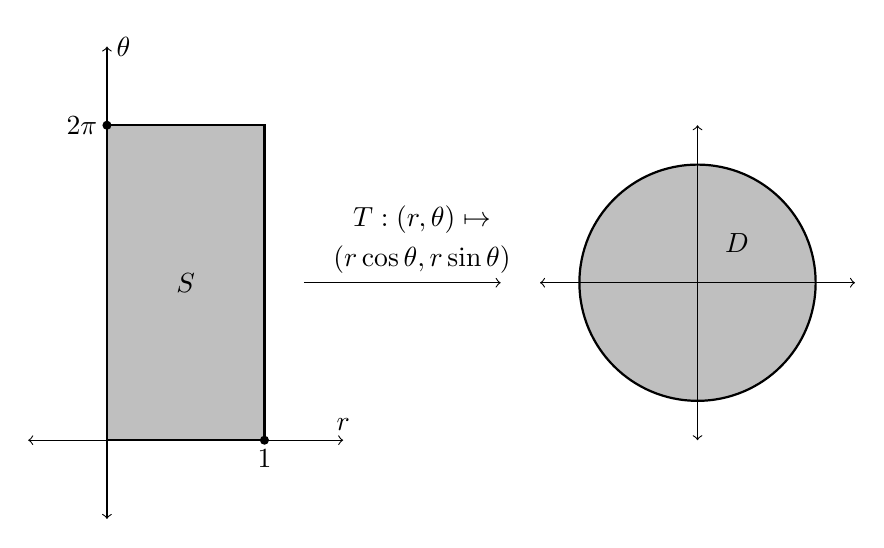
\begin{tikzpicture}
      \draw[thick, fill=lightgray] (7.5,2) circle (1.5);
      \draw[<->] (-1,0)--(3,0);
      \draw[<->] (0,-1)--(0,5);
      \draw[thick, fill=lightgray] (0,0) rectangle (2,4);
      \node at (1,2) {$S$};
      \draw[fill] (0,4) circle (0.05);
      \draw[fill] (2,0) circle (0.05);
      \node[below] at (2,0) {$1$};
      \node[left] at (0,4) {$2 \pi$};
      \node[above] at (3,0) {$r$};
      \node[right] at (0,5) {$\theta$};
      \draw[->] (2.5, 2)--(5,2);
      \node[above] at (4,2.5) {$T: (r, \theta) \mapsto$};
      \node[above] at (4,2) {$ (r \cos{\theta}, r \sin{\theta})$};
      \draw[<->] (5.5,2)--(9.5,2);
      \draw[<->] (7.5,0)--(7.5,4);
      \node at (8,2.5) {$D$};
  \end{tikzpicture}  
  \end{center}
  \end{example}

  \begin{theorem}[Integration over Change of Bases in $\mathbb{R}^n$]
    Let $\mathbb{R}^n$ have the standard orthonormal basis $e_1, e_2, ..., e_n$, and let us construct a new basis $f_1, f_2, ..., f_n$ such that the coefficients of the vectors in $\mathbb{R}^n$ are related with the functions
    \[B: \mathbb{R}^n \longrightarrow \mathbb{R}^n, \;\;\;\; B(u_1, u_2, \ldots, u_n) = \begin{pmatrix}
    x_1 (u_1, \ldots, u_n) \\x_2 (u_1, \ldots, u_n) \\ \vdots \\ x_n (u_1, \ldots, u_n)
    \end{pmatrix}\]
    Given that the region $D \subset \mathbb{R}^n$ is transformed into a new region $S = B(D) \subset \mathbb{R}^n$ under this basis transformation, the integral of function $f(x_1, \ldots, x_n)$ over region $D$ can be expressed as 
    \[\int_D f(x) \, dH = \int_S f \big( x_1(u), x_2(u), ..., x_n (u) \big) \big| J B(u_1, \ldots, u_n)\big| \, d \bar{H}\]
    where the integral on both the left and right hand side represents integration over an $n$-dimensional region, $x$ represents the $n$-tuple $(x_1, \ldots, x_n)$, $u$ represents the $n$-tuple $(u_1, \ldots, u_n)$, and $\big| J B(u_1, \ldots, u_n)\big|$ represents the Jacobian determinant of function $B$. 
  \end{theorem}

  We now describe some common change of basis formulas for polar, cylindrical, and spherical coordinates. 

  \begin{theorem}[Integration in Polar Coordinates]
    \begin{equation}
      \iint_{D} f(x, y) \, dx \,dy = \iint_S f(r \cos{\theta}, r \sin{\theta}) r \, dr \, d\theta
    \end{equation}
  \end{theorem}

  \begin{definition}[Cylindrical, Spherical Coordinates]
  In $\mathbb{R}^3$, \textit{cylindrical coordinates} have the following relation to rectangular coordinates. 
  \begin{align}
      & x = r \cos{\theta} \\
      & y = r \sin{\theta} \\
      & z = z
  \end{align}
  In $\mathbb{R}^3$, \textit{spherical coordinates} have the following relation to rectangular coordinates. 
  \begin{align*}
      & x = \rho \sin{\phi} \cos{\theta} \\
      & y = \rho \sin{\phi} \sin{\theta} \\
      & z = \rho \cos{\phi}
  \end{align*}
  \end{definition}

  \begin{corollary}[Integration in Cylindrical Coordinates]
  \[\iiint_D f(x, y, z) \, dx \, dy \, dz = \iiint_S f( r \cos{\theta}, r \sin{\theta}, z) r \, dr \, d\theta \, dz\]
  \end{corollary}

  \begin{corollary}[Integration in Spherical Coordinates]
  \[\iiint_D f(x, y, z) \,dx\,dy\,dz = \iiint_S f(\rho \sin{\phi} \cos{\theta}, \rho \sin{\phi} \sin{\theta}, \rho \cos{\phi}) \rho^2 \sin{\theta} \, d\rho \, d\theta \, d\phi\]
  \end{corollary}

  \begin{example}[Gaussian Integral]
  The following is the (un-normalized) probability distribution function of the Gaussian distribution. 
  \[\int_{-\infty}^{\infty} e^{-x^2} \, dx = \sqrt{\pi}\]
  \end{example}

\subsection{Improper Integrals}

  There are generally two types of improper integrals. 
  \begin{enumerate}
    \item The region $D$ integrated over is unbounded. 
    \item The function $f$ that is integrated is unbounded within the region $D$.
  \end{enumerate}

  These types of improper integrals are usually evaluated using a limiting process. When the interval $I$ is unbounded, say $(1, \infty)$, the integral can be evaluated as 
  \[\int_1^\infty \frac{1}{x^2} \,dx = \lim_{b \rightarrow \infty} \int_1^b \frac{1}{x^2} \, dx = \lim_{b\rightarrow \infty} \bigg( 1 - \frac{1}{b} \bigg) = 1\]
  In case 2, we can add a limit at the point where the function $f$ diverges as such. 
  \[\int_0^1 \frac{1}{\sqrt{x}} \, dx = \lim_{a \rightarrow 0} \int_a^1 \frac{1}{\sqrt{x}} \, dx = \lim_{a \rightarrow 0} (2 - 2\sqrt{a}) = 2\]
  We now describe how to integrate over a certain path $p$ embedded in a higher dimensional space $\mathbb{R}^n$, possibly with a scalar or vector field $f$. We must first go over oriented paths. 

  Extending the previous case, we use a multivariate limiting process in $\mathbb{R}^2$. We will first work with case 2, when $f$ is unbounded within the region $D$. Let us define an elementary region $D$ in $\mathbb{R}^2$; without loss of generality, we will make it $y$-simple, meaning that $D$ can be expressed as
    \[D \equiv \{ (x, y) \in \mathbb{R}^2 \; | \; a \leq x \leq b, \; \phi_1 (x) \leq y \leq \phi_2 (x)\}\]
  We can actually assume that the region in which $f$ is unbounded lies in the boundary $\partial D$. This is because if it lied in the interior of $D$, we could split $D$ into pieces across a path that intersects this region with divergent values, evaluate the integrals over the pieces separately, and then sum the integrals. For example, in the rectangular region below, let the dashed line represent the values where the function $f$ diverges. Then, we can split the region into two rectangular regions shown in the right. 
  \begin{center}
  \begin{tikzpicture}
    \draw (0,0) rectangle (3,2);
    \draw[dashed] rectangle (2,0)--(2,2);
    \draw[->] (3.5,1)--(5,1);
    \draw (8,0)--(6,0)--(6,2)--(8,2);
    \draw[dashed] (8,0)--(8,2);
    \draw[dashed] (9,0)--(9,2);
    \draw (9,0)--(10,0)--(10,2)--(9,2);
  \end{tikzpicture}
  \end{center}
  Therefore, assuming that $f$ is unbounded in $\partial D$, we can construct a new region 
  \[D_{\eta, \delta} \equiv \{(x, y) \in \mathbb{R}^2 \; | \; a + \eta \leq x \leq b - \eta, \; \phi_1 (x) + \delta \leq y \leq \phi_2 (x) - \delta\}\]
  for some arbitrarily small numbers $\eta, \delta >0$, meaning that the integral (reduced to iterated integrals using Fubini's theorem) 
  \[F(\eta, \delta) \equiv \iint_{D_{\eta, \delta}} f(x, y) \, dA = \int_{a + \eta}^{b - \eta} \int_{\phi_1 (x) + \delta}^{\phi_2 (x) - \delta} f(x, y) \, dy\,dx\]
  is well defined. 
  \begin{center}
  \begin{tikzpicture}
      \draw[<->] (-0.5,0)--(5,0);
      \draw[<->] (0,-0.5)--(0,5);
      \draw (1,1.5)--(1,3);
      \draw plot [smooth] coordinates {(1,3) (1.5,3.3) (2,3.1) (3,3.8) (4,4.2) (4.5,4)};
      \draw (4.5, 4)--(4.5,1);
      \draw plot [smooth] coordinates {(1,1.5) (2,1.7) (3, 1.6) (3.7, 1.3) ( 4.5,1)};
      \draw[dashed] (1.3,1.85)--(1.3,2.9);
      \draw[dashed] (4.2, 3.8)--(4.2,1.4);
      \draw[dashed] plot [smooth] coordinates {(1.3,2.9) (1.5,3) (2,2.8) (3,3.5) (4,3.9) (4.2,3.8)};
      \draw[dashed] plot [smooth] coordinates {(1.3,1.85) (2,2) (3, 1.9) (3.7, 1.6) ( 4.2,1.4)};
      \node at (3,2.5) {$D_{\eta, \delta}$};
      \node[below left] at (2,1) {$D$};
      \draw[->] (2,1)--(2.5,1.85);
  \end{tikzpicture}
  \end{center}
  Clearly, the function $F( \eta, \delta)$ is a function of two variables $\eta$ and $\delta$. So, if the limit 
  \[\lim_{(\eta, \delta) \rightarrow (0, 0)} F(\eta, \delta)\]
  is well defined, then so is the improper integral. For it to exist, the iterated limits must both equal to a well-defined real number $\mathcal{L}$ (and to each other). That is, 
  \[\lim_{\eta \rightarrow 0} \lim_{\delta \rightarrow 0} F(\eta, \delta) = \lim_{\delta \rightarrow 0} \lim_{\eta \rightarrow 0} F(\eta, \delta) = \mathcal{L} \implies \lim_{(\eta, \delta) \rightarrow (0,0)} F(\eta, \delta) = \mathcal{L}\]


  It is also worthwhile to note that functions unbounded at isolated points can be evaluated using the methods above using a change of basis. Consider the example below. 

  \begin{example}
  In the unit disk $D \subset \mathbb{R}^2$, let the function $f$ be defined as 
  \[f(x, y) \equiv \frac{1}{\sqrt{x^2 + y^2} }\]
  Clearly, $f$ is continuous at every point except $0= (0,0)$, meaning that 
  \[\iint_{D \setminus \{0\}} f(x, y)\, dA\]
  is well-defined. In order to solve the integral over the entire disk, we convert to polar coordinates and evaluate the limit
  \[\iint_{D \setminus \{0\}} f(x, y) \, dA = \lim_{\delta \rightarrow 0} \int_{\delta}^1 \int_0^{2 \pi} r \, f( r \cos{\theta}, r \sin{\theta}) \, d\theta \,dr\]
  \end{example}
  \begin{center}
  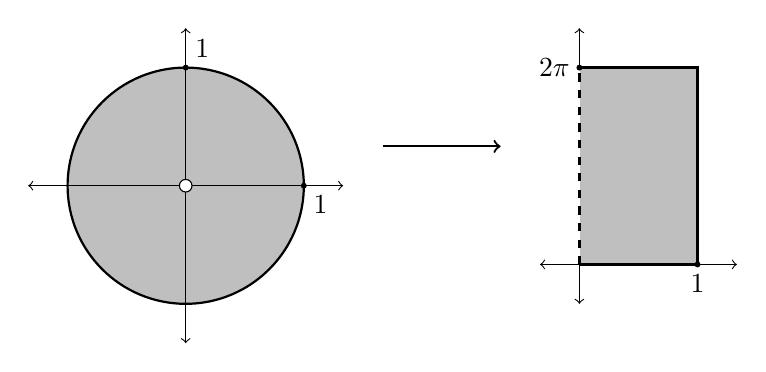
\begin{tikzpicture}
      \draw[thick, fill=lightgray] (0,0) circle (1.5); 
      \draw[<->] (-2,0)--(2,0);
      \draw[<->] (0,-2)--(0,2);
      \draw[fill=white] (0,0) circle (0.08);
      \draw[->, thick] (2.5,0.5)--(4, 0.5); 
      \draw[<->] (4.5,-1)--(7,-1);
      \draw[<->] (5,-1.5)--(5,2);
      \draw[white, fill=lightgray] (5,-1) rectangle (6.5,1.5);
      \draw[thick] (5,-1)--(6.5,-1)--(6.5,1.5)--(5,1.5);
      \draw[thick, dashed] (5,-1)--(5,1.5);
      \draw[fill] (6.5,-1) circle (0.03);
      \node[below] at (6.5,-1) {$1$};
      \node[left] at (5,1.5) {$2 \pi$};
      \draw[fill] (5, 1.5) circle (0.03);
      \draw[fill] (1.5,0) circle (0.03);
      \draw[fill] (0,1.5) circle (0.03);
      \node[below right] at (1.5,0) {$1$};
      \node[above right] at (0,1.5) {$1$};
  \end{tikzpicture}
  \end{center}

  If we are given an unbounded region $D \subset \mathbb{R}^2$, we can first create a bounded region and expand that region using a limit to cover all of $D$. 
